\documentclass[aspectratio=169,10pt]{beamer}

\usetheme{Madrid}
\usecolortheme{seahorse}
\setbeamertemplate{footline}[frame number]

\usepackage[utf8]{inputenc}
\usepackage[T1]{fontenc}
\usepackage{amsmath, amssymb, amsfonts}
\usepackage{mathtools}
\usepackage{xcolor}
\usepackage{graphicx}
\usepackage{listings}
\usepackage{xfrac}
\usepackage{array}
\usepackage{adjustbox}

\graphicspath{{figures/}}

% Define colors for listings
\definecolor{mygreen}{rgb}{0, 0.6, 0}
\definecolor{mygray}{rgb}{0.5, 0.5, 0.5}
\definecolor{mymauve}{rgb}{0.58, 0, 0.82}

\lstset{
    basicstyle=\ttfamily\scriptsize,
    commentstyle=\color{mygreen}\itshape,
    keywordstyle=\color{blue},
    stringstyle=\color{mymauve},
    breaklines=true,
    breakatwhitespace=true,
    tabsize=2,
    numbers=left,
    numbersep=5pt,
    frame=single,
    framerule=0.5pt,
    backgroundcolor=\color{gray!10},
    showspaces=false,
    showtabs=false,
    extendedchars=true,
    language=Python
}

% Mathematical notation
\newcommand{\norm}[1]{\left\lVert #1 \right\rVert}
\newcommand{\abs}[1]{\left\lvert #1 \right\rvert}
\newcommand{\set}[1]{\left\{ #1 \right\}}
\newcommand{\ip}[2]{\left\langle #1, #2 \right\rangle}
\newcommand{\spa}[1]{\overline{#1}}
\newcommand{\dpart}[2]{\frac{\partial #1}{\partial #2}}

\title{Chapter 6: Degree Theory, k-Set Contractions and Condensing Operators}
\subtitle{Nonlinear Analysis and Fixed Point Theory}
\author{Pathak (2018)}
\date{Pages 495--516}

\begin{document}

\frame{\titlepage}

% ============================================================================
\begin{frame}{Table of Contents}
  \tableofcontents
\end{frame}

% ============================================================================
\section{6.2 Degree Theory: Invariance Principles}
% ============================================================================

\begin{frame}{6.2.1 Invariance Principles in Degree Theory}

\textbf{Challenge:} When defining a completely continuous vector field $\Phi = I - A$ in infinite-dimensional Banach spaces, the choice of Banach space is crucial. The geometric properties depend heavily on this choice.

\vspace{0.5cm}

\textbf{Question:} If $\Phi = I - A$ is completely continuous in two different Banach spaces $X_1$ and $X_2$, how do the rotation numbers $\gamma(\Phi, \Omega_i, 0)$ relate?

\vspace{0.5cm}

\textbf{Key Definitions:}
\begin{itemize}
    \item \alert{Common core}: Sets $\Omega_1 \subset X_1$ and $\Omega_2 \subset X_2$ have a common core if the fixed points of $A$ in the closures of $\Omega_1$ and $\Omega_2$ coincide
    \item \alert{Compatible norms}: When embedding spaces, the norm structures preserve key properties
    \item \alert{Condition $\alpha_0(\partial\Omega)$}: Technical condition ensuring continuity properties of the vector field on the boundary
\end{itemize}

\end{frame}

\begin{frame}{Main Invariance Principles}

\begin{theorem}[6.19 - Invariance Theorem]
Let $X_1$ and $X_2$ be Banach spaces with $\Omega_1 \subset X_1$, $\Omega_2 \subset X_2$ bounded open sets. Assume $\Phi = I - A$ is completely continuous on $\Omega_1$ and $\Omega_2$ with:

\textbf{Case (a):} $A$ continuous on $\overline{\Omega}_1, \overline{\Omega}_2$ as an operator $X_i \to X_i$.

\textbf{Case (b):} Norms are compatible; $A$ is locally bounded and compact.

\textbf{Case (c):} Norms compatible; $\exists$ compact convex sets $S_1 \subset X_1 \cap X_2$, with $A(S_1 \cap \Omega_1) \subset S_2$ and $A(S_2 \cap \Omega_2) \subset S_1$.

Then: $\gamma(\Phi, \Omega_1) = \gamma(\Phi, \Omega_2)$
\end{theorem}

\textbf{Interpretation:} The degree is independent of the choice of Banach space (under suitable conditions).

\end{frame}

\begin{frame}[fragile]{Index Formula and Rotation}

\textbf{Computing the Index:} If $\Omega$ is bounded and $N(\Phi, \Omega)$ (zeros of $\Phi$ in $\overline{\Omega}$) is finite $\{x_0, \ldots, x_s\}$:

\[
\gamma(\Phi, \Omega) = \text{ind}(x_0, \Phi) + \cdots + \text{ind}(x_s, \Phi)
\]

where $\text{ind}(x_i, \Phi)$ is the local index at an isolated zero.

\vspace{0.4cm}

\textbf{Example (Equation 6.13):}
\begin{lstlisting}
# Python: Computing index for vector field at origin
import numpy as np

def vector_field(x, y):
    """Phi(x,y) = (x - f1(x,y), y - f2(x,y))"""
    return np.array([x - 0.1*x*y, y + 0.05*x**2])

# Evaluate on boundary of Omega
theta = np.linspace(0, 2*np.pi, 1000)
x_boundary = 2 * np.cos(theta)
y_boundary = 2 * np.sin(theta)
phi_vals = [vector_field(x, y) for x, y in zip(x_boundary, y_boundary)]

# Index ~ winding number around origin
\end{lstlisting}

\begin{center}
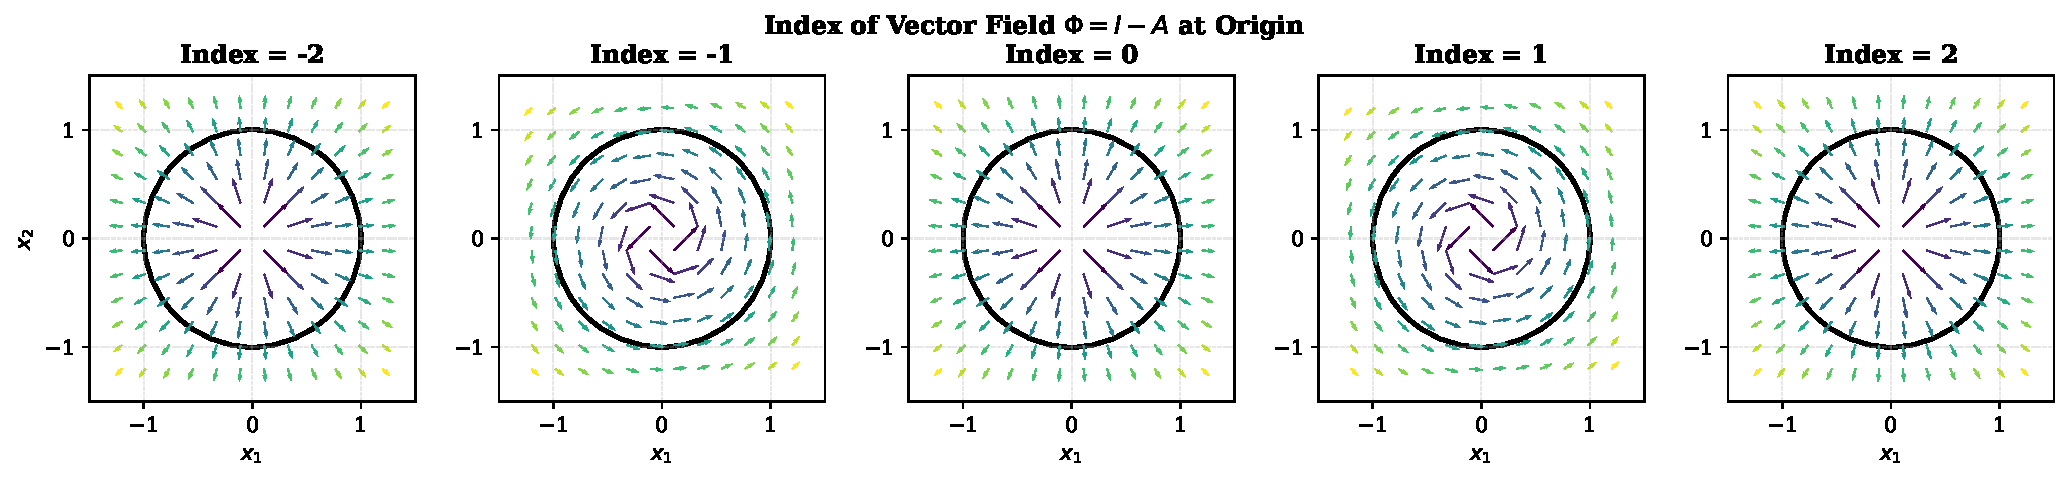
\includegraphics[width=0.6\textwidth]{fig_vector_field_index}
\end{center}

\end{frame}

% ============================================================================
\section{6.3 The Skrypnik Degree Theory}
% ============================================================================

\begin{frame}{6.3 Introduction to Skrypnik Degree Theory}

\textbf{Skrypnik's 1973 monograph} developed a new topological degree theory for mappings:
\begin{itemize}
    \item From a reflexive space $X$ to its dual $X^*$
    \item Class $\alpha$ operators (including demicontinuous and pseudomonotone)
    \item Applications to solvability of nonlinear elliptic PDEs
\end{itemize}

\vspace{0.3cm}

\textbf{Important cases:}
\begin{enumerate}
    \item $\Gamma = X^*$ (general case)
    \item $X$ reflexive, $\Gamma = X^*$ (standard)
    \item $X = Z^*$ where $Z$ is Banach, $\Gamma = Z \subseteq X^{**}$
\end{enumerate}

\vspace{0.4cm}

\textbf{Key technical aspect:} For operators $\Phi: \mathfrak{M} \to X^*$ with $\mathfrak{M} \subset X$:
\begin{itemize}
    \item $\langle u, v \rangle$ denotes the action of the functional $u \in X^*$ on $v \in X$
    \item Weak and strong convergence denoted by $\rightharpoonup$ and $\to$ respectively
\end{itemize}

\end{frame}

\begin{frame}{Definition of Class $\alpha$ Operators}

\begin{definition}[Class $\alpha$ - Definition 6.6]
An operator $\Phi: \mathfrak{M} \to X^*$ satisfies \alert{condition $\alpha(\mathfrak{M})$} if:
\[
\limsup_{n \to \infty} \langle \Phi(x_n), x_n - x_0 \rangle \leq 0
\]
for any sequence $x_n \in \mathfrak{M}$ with $x_n \rightharpoonup x_0$.

This is satisfied when:
\end{definition}

\begin{itemize}
    \item $\Phi$ is \textbf{pseudomonotone}: If $x_n \rightharpoonup x_0$ and $\limsup \langle \Phi(x_n), x_n - x_0 \rangle \leq 0$, then for all $v$:
    \[
    \liminf_{n \to \infty} \langle \Phi(x_n), x_n - v \rangle \geq \langle \Phi(x_0), x_0 - v \rangle
    \]

    \item $\Phi$ is \textbf{demicontinuous} and monotone

    \item $\Phi$ is \textbf{completely continuous} on reflexive spaces
\end{itemize}

\end{frame}

\begin{frame}{Skrypnik Degree Definition}

\begin{theorem}[6.22 - Skrypnik Degree Definition]
Let $\Omega$ be a bounded open set in reflexive Banach space $X$, and $A: \bar{\Omega} \to X^*$ a demicontinuous pseudomonotone operator with:
\[
\|Au\|_{X^*} \geq \delta_0 > 0 \quad \text{for all } u \in \partial\Omega
\]

If $0 \notin A(\partial\Omega)$, the \alert{Skrypnik degree}
\[
\deg(A, \Omega, 0) = \lim_{n \to \infty} \deg(A_n, \Omega_n, 0)
\]
is well-defined, where $A_n = P_n A|_{F_n}$ are finite-dimensional restrictions.
\end{theorem}

\vspace{0.3cm}

\textbf{Key properties:}
\begin{itemize}
    \item The degree exists and is independent of the finite-dimensional approximation
    \item Satisfies homotopy invariance under suitable conditions
    \item $\deg(A, \Omega, 0) \neq 0 \Rightarrow$ existence of solutions to $Au = u$ in $\Omega$
\end{itemize}

\end{frame}

\begin{frame}[fragile]{Skrypnik Degree Conditions}

\begin{center}
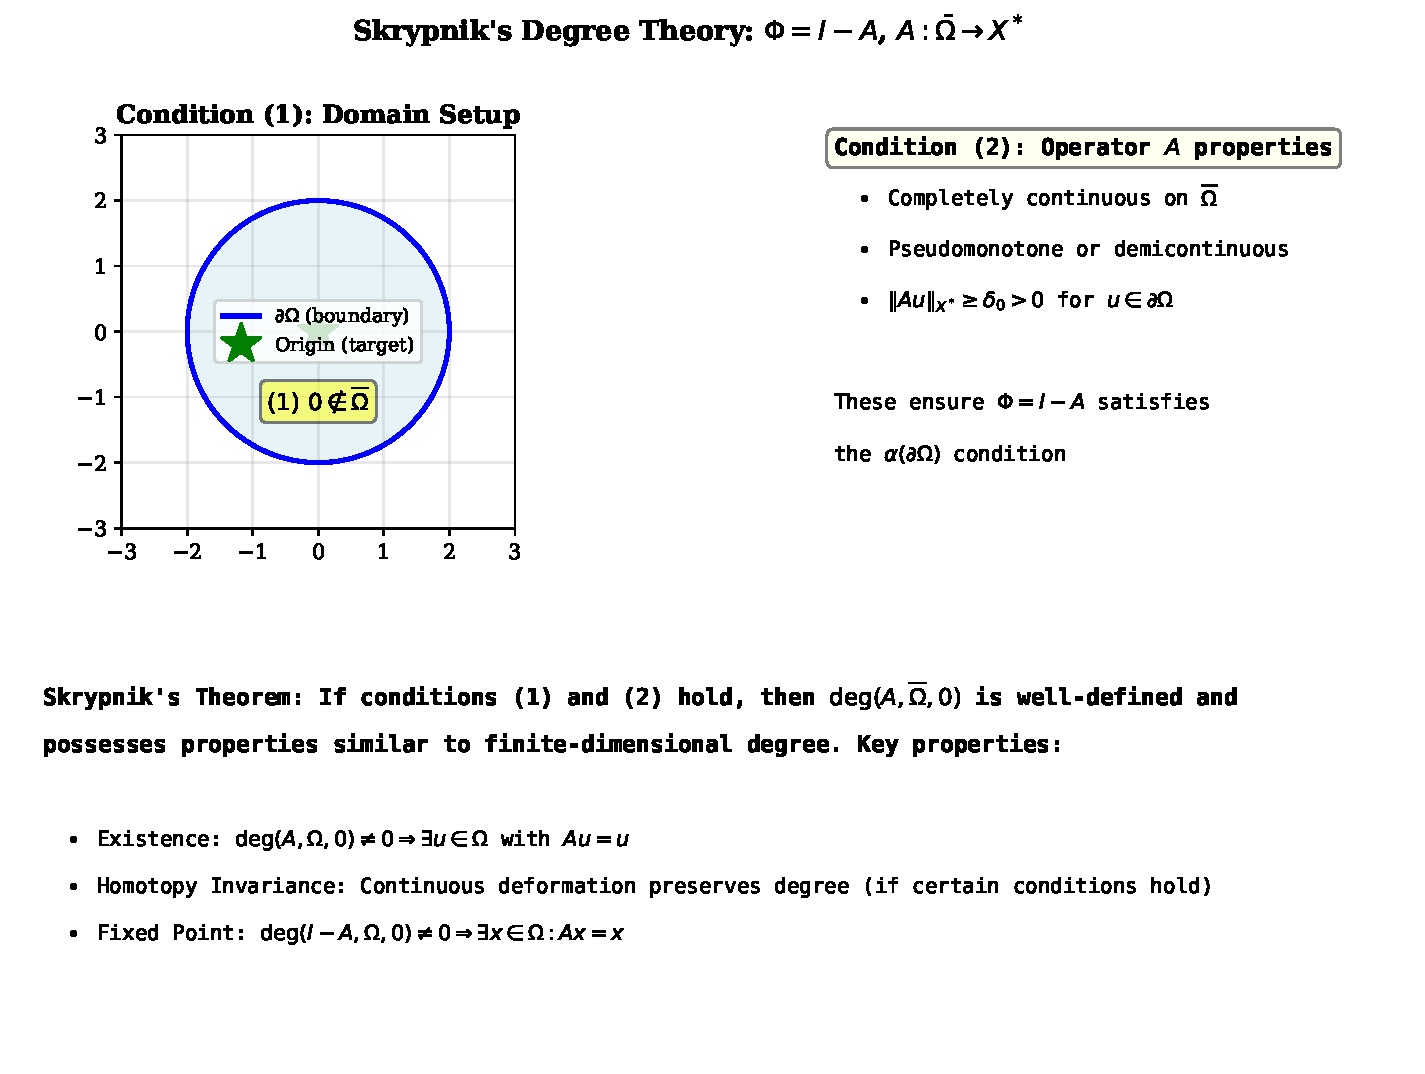
\includegraphics[width=0.95\textwidth]{fig_skrypnik_degree}
\end{center}

\textbf{Main conditions (Theorem 6.22):}
\begin{enumerate}
    \item \textbf{Condition (1):} $0 \notin \overline{\Omega}$ (zero not in closure)
    \item \textbf{Condition (2):} Operator $A$ is:
    \begin{itemize}
        \item Completely continuous on $\overline{\Omega}$
        \item Pseudomonotone or demicontinuous
        \item Bounded away from zero: $\|Au\|_{X^*} \geq \delta_0$
    \end{itemize}
\end{enumerate}

\end{frame}

\begin{frame}{Approximation and Convergence}

\textbf{Key Lemma (for proving Skrypnik's theorem):}

When approximating $A$ by finite-dimensional restrictions $A_n$ on subspaces $F_n$:

\begin{equation}
\lim_{n \to \infty} \deg(A_n, \Omega_n, 0) = \deg(A, \Omega, 0) \quad \text{(independent of sequence)}
\end{equation}

\vspace{0.3cm}

\textbf{Proof strategy:}
\begin{enumerate}
    \item Use the fact that finite-dimensional degree is well-established
    \item $[tA_n + (1-t)\tilde{A}_n]u \neq 0$ for $u \in \partial\Omega_n$, $t \in [0,1]$ (homotopy condition)
    \item As $n \to \infty$, the degress stabilize to the infinite-dimensional degree
\end{enumerate}

\vspace{0.3cm}

\textbf{Remark 6.7:} The Skrypnik degree shares essential properties with the Leray-Schauder degree but applies to a broader class of operators (pseudomonotone, not just compact).

\end{frame}

% ============================================================================
\section{6.4 k-Set Contractions}
% ============================================================================

\begin{frame}{6.4.1 k-Set Contractions: Definition and Properties}

\begin{definition}[k-Set Contraction]
A mapping $T: X \to X$ is a \alert{k-set contraction} if:
\[
\mu(T(A)) \leq k \cdot \mu(A)
\]
for every bounded set $A \subseteq X$, where $\mu$ is the \textbf{measure of noncompactness} and $k \in [0, 1)$.
\end{definition}

\vspace{0.3cm}

Special cases:
\begin{itemize}
    \item $k = 0$: \textbf{Compact operator} (image has measure zero)
    \item $k = 1$: \textbf{Nonexpansive mapping} in the measure sense
    \item $0 < k < 1$: Strict contraction on the measure of noncompactness
\end{itemize}

\vspace{0.3cm}

\textbf{Example 6.4:} The measure of noncompactness can be defined as:
\[
\mu(A) = \inf\{\epsilon > 0 : A \text{ can be covered by finitely many balls of radius } \epsilon\}
\]

\begin{center}
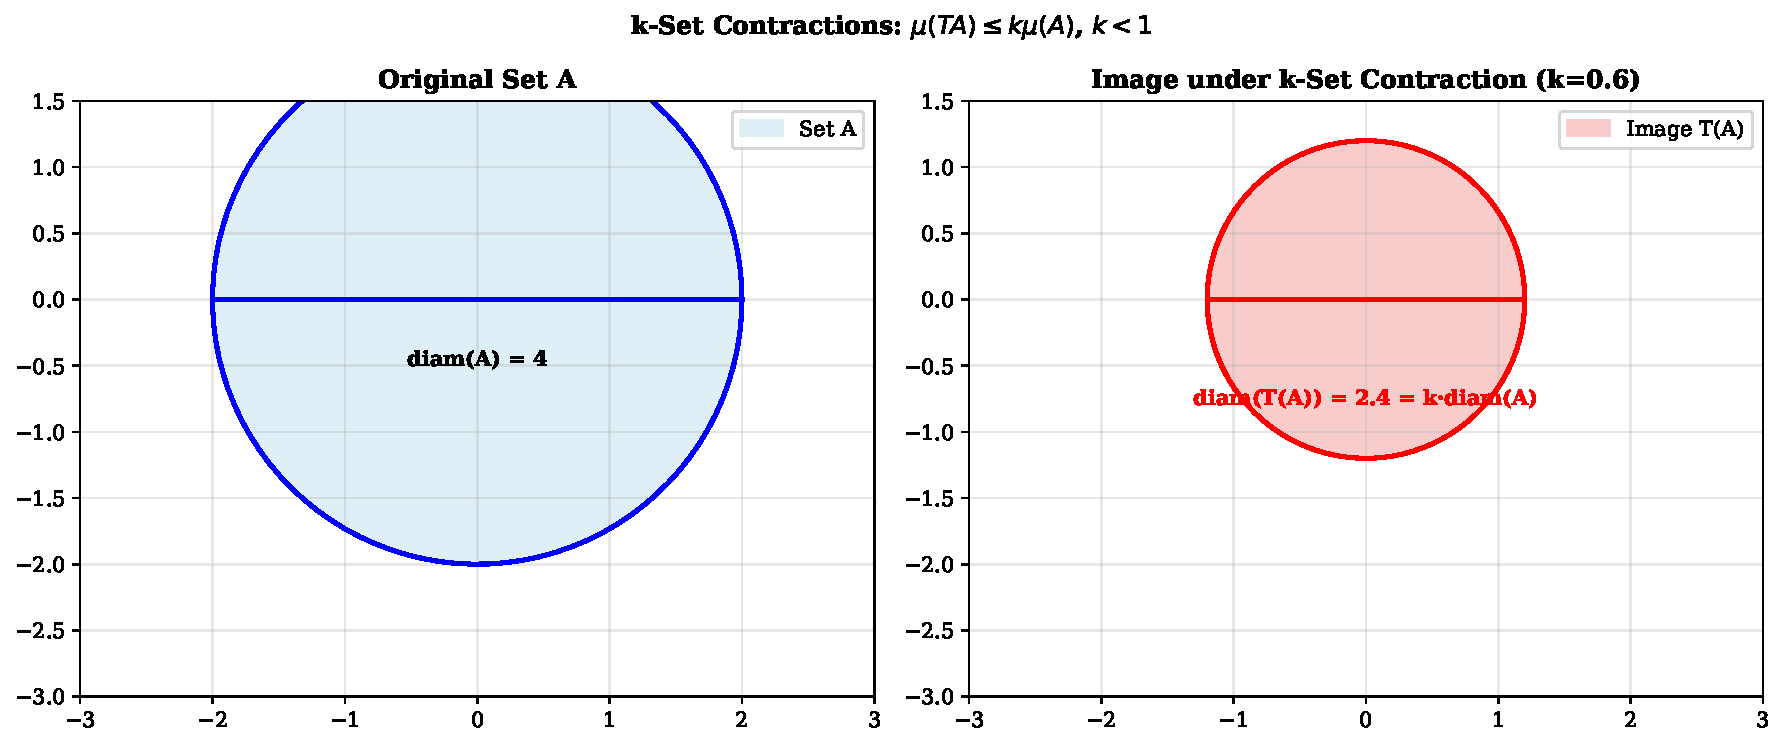
\includegraphics[width=0.8\textwidth]{fig_k_set_contractions}
\end{center}

\end{frame}

\begin{frame}{Measure of Noncompactness: Kuratowski Measure}

\begin{definition}[Kuratowski Measure of Noncompactness]
For a bounded set $A$ in a metric space $(X, d)$:
\[
\alpha(A) = \inf\left\{\epsilon > 0 : A \text{ has a finite covering by sets of diameter} \leq \epsilon\right\}
\]
\end{definition}

\textbf{Key properties:}
\begin{enumerate}
    \item \textbf{Monotonicity}: $A \subseteq B \Rightarrow \alpha(A) \leq \alpha(B)$
    \item \textbf{Regularity}: $\alpha(A) = 0 \Leftrightarrow A$ is \textit{compact}
    \item \textbf{Additivity}: $\alpha(A \cup B) = \max\{\alpha(A), \alpha(B)\}$
    \item \textbf{Subadditivity}: $\alpha(A + B) \leq \alpha(A) + \alpha(B)$ (Minkowski sum)
    \item \textbf{Homogeneity}: $\alpha(\lambda A) = |\lambda| \alpha(A)$
\end{enumerate}

\vspace{0.3cm}

\textbf{Hausdorff measure}: Related but defined via $\epsilon$-coverings in terms of the number of balls.

\vspace{0.3cm}

\begin{center}
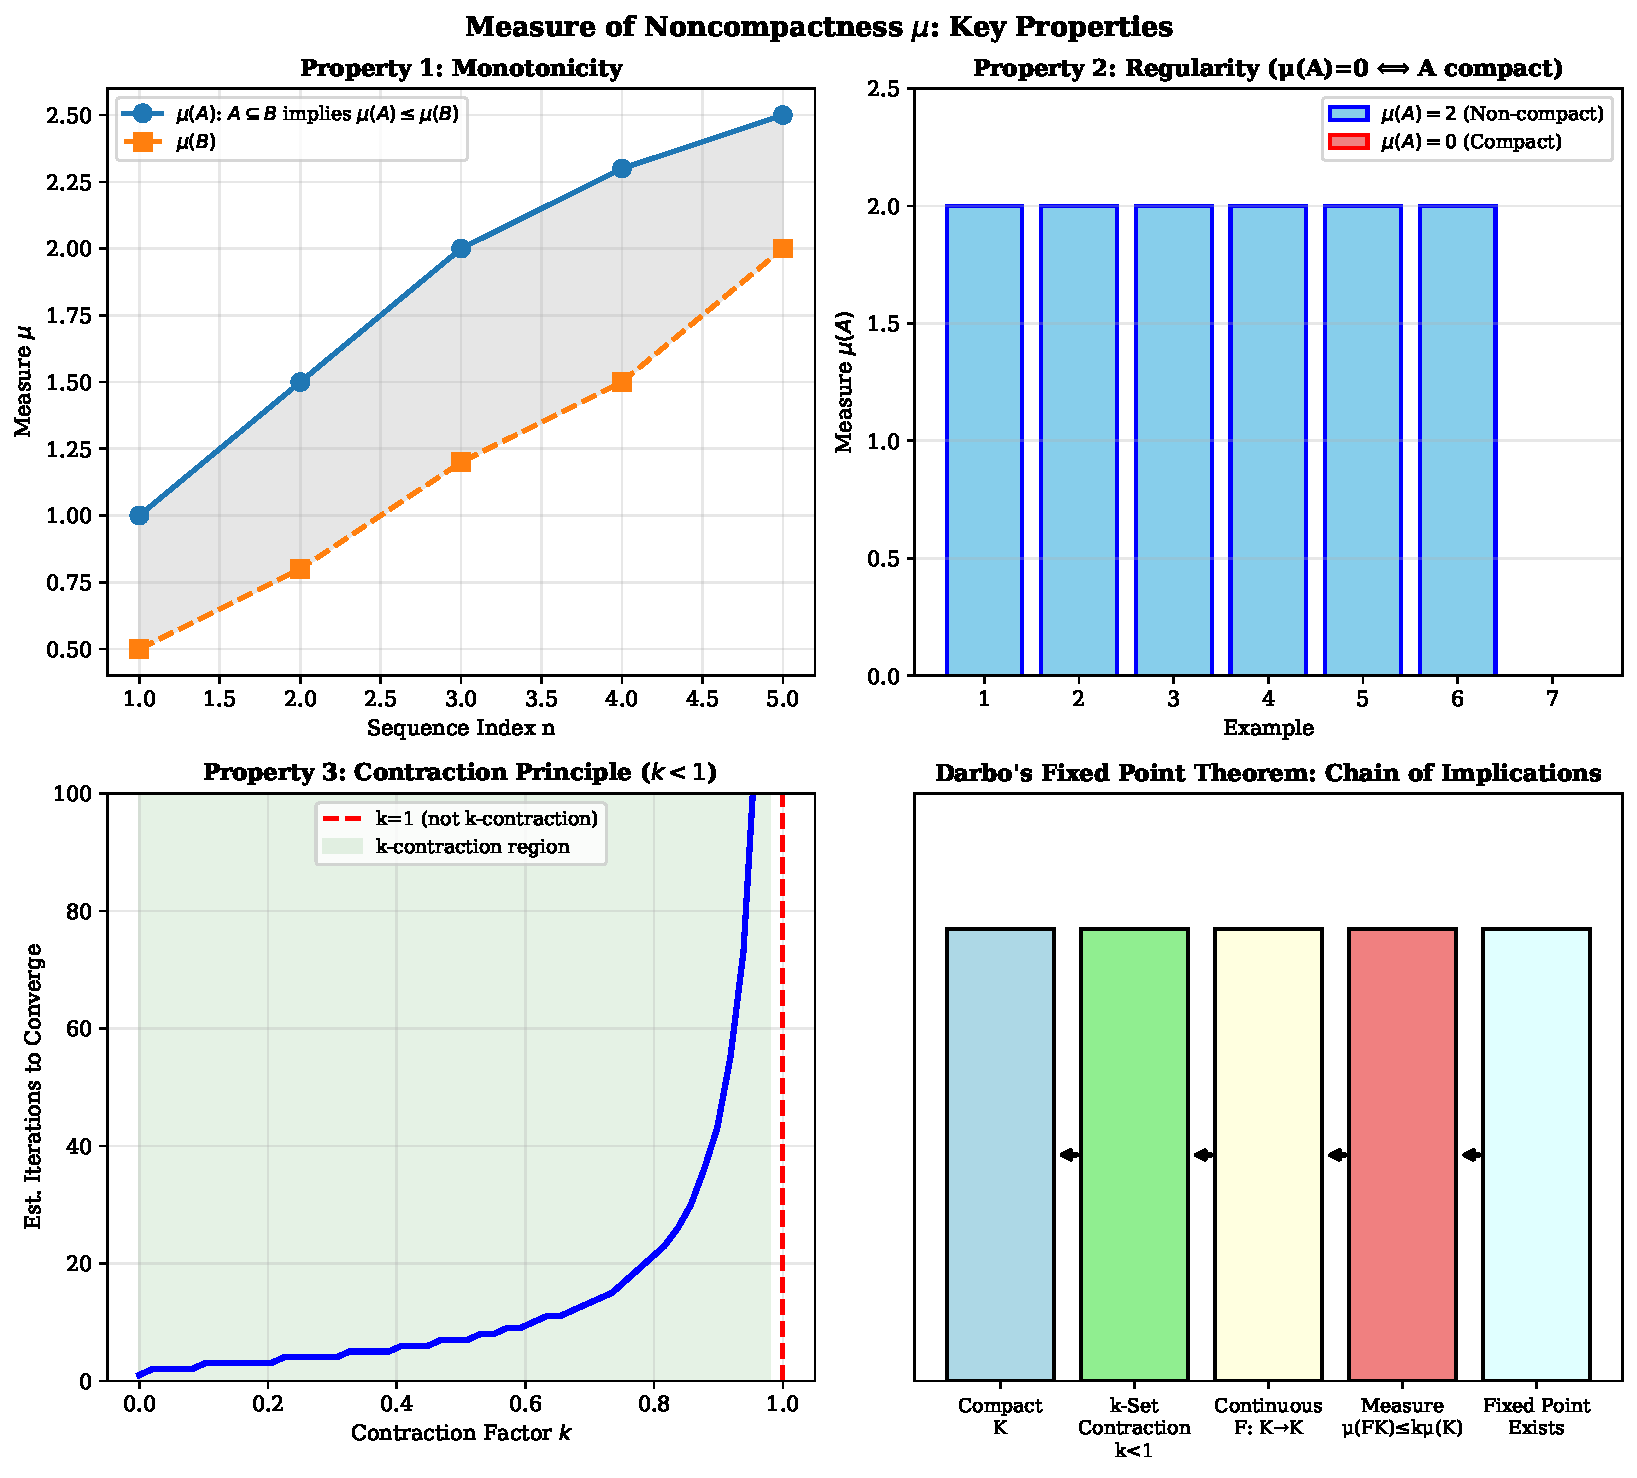
\includegraphics[width=0.7\textwidth]{fig_measure_noncompactness}
\end{center}

\end{frame}

\begin{frame}[fragile]{Properties of Measure of Noncompactness}

\textbf{Fundamental Theorem:} For any bounded set $A$ and continuous operator $T$:

\[
\alpha(T(A)) \leq \text{diam}(T(A))
\]

\textbf{Theorem 6.23 (Darbo)}: If $T: \Omega \to \Omega$ is continuous on bounded closed convex set $\Omega$ with:
\[
\mu(T(X)) \leq k \cdot \mu(X) \quad \text{for some } k < 1
\]
then $T$ has a fixed point in $\Omega$.

\vspace{0.5cm}

\textbf{Code Example: Computing Measure of Noncompactness}

\begin{lstlisting}
# Estimate measure of noncompactness via covering
def measure_noncompactness(points, epsilon_tolerance=0.01):
    """Compute approximate Kuratowski measure"""
    from scipy.spatial.distance import pdist, squareform

    dists = squareform(pdist(points))
    # Greedy covering algorithm
    covered = set()
    num_balls = 0
    for i in range(len(points)):
        if i not in covered:
            num_balls += 1
            # Find all points within epsilon
            neighbors = np.where(dists[i] <= epsilon_tolerance)[0]
            covered.update(neighbors)

    return num_balls, epsilon_tolerance
\end{lstlisting}

\end{frame}

\begin{frame}{Darbo's Fixed Point Theorem}

\begin{theorem}[6.24 - Darbo]
Let $\Omega$ be a nonempty, bounded, closed and convex subset of a Banach space $E$, and let $T: \Omega \to \Omega$ be a continuous mapping. If there exists a constant $k \in [0, 1)$ such that:
\[
\mu(T(X)) \leq k \cdot \mu(X)
\]
for any nonempty subset $X \subseteq \Omega$, where $\mu$ is the measure of noncompactness, then $T$ has a fixed point in $\Omega$.
\end{theorem}

\vspace{0.3cm}

\textbf{Key observations:}
\begin{enumerate}
    \item Generalizes Banach Contraction Principle to infinite dimensions
    \item Does not require $T$ to be a contraction in the usual sense ($\|Tx - Ty\| \leq k\|x - y\|$)
    \item Uses measure of noncompactness instead of pointwise distance
\end{enumerate}

\vspace{0.3cm}

\textbf{Remark:} If $K$ is compact or $F$ is compact, Theorem 5.24 (Schauder) is a special case. If $K$ is compact and $F$ is weakly continuous in reflexive Banach space, this is the Tychonoff fixed point theorem.

\end{frame}

\begin{frame}{Nonlinear k-Set Contractions}

\begin{definition}[Nonlinear k-Set Contraction]
A mapping $T: X \to X$ is a \alert{nonlinear k-set contraction} if there exists a continuous $\varphi: \mathbb{R}^+ \to \mathbb{R}^+$ with $\varphi(0) = 0$ such that:
\[
\mu(T(A)) \leq \varphi(\mu(A)) \quad \text{for all bounded } A \subseteq X
\]
where $\varphi(r) < r$ for all $r > 0$.
\end{definition}

\vspace{0.3cm}

Examples of $\varphi$ functions:
\begin{itemize}
    \item \textbf{Linear}: $\varphi(r) = kr$ with $k < 1$ (standard k-set contraction)
    \item $\varphi(r) = \frac{kr}{1+r}$ with $L > 0$, $K > 0$
    \item $\varphi(r) = \log(1 + r)$
\end{itemize}

\vspace{0.3cm}

\begin{lemma}[6.9 - Limit Behavior]
If $\varphi$ is a $\varphi$-function on $\mathbb{R}^+$ into itself with $\varphi(r) < r$ for $r > 0$, then:
\[
\lim_{n \to \infty} \varphi^n(t) = 0 \quad \text{for all } t \in [0, \infty)
\]
\end{lemma}

\end{frame}

% ============================================================================
\section{6.5 Condensing Operators}
% ============================================================================

\begin{frame}{Condensing Operators: Definition}

\begin{definition}[$\alpha$-Condensing Operator]
A continuous mapping $T: \Omega \to X$ is called $\alpha$-\alert{condensing} if for every nonempty bounded set $A \subseteq \Omega$:
\[
\alpha(T(A)) < \alpha(A)
\]
where $\alpha$ is the measure of noncompactness, \textbf{unless} $A$ is compact (in which case $\alpha(A) = 0$).
\end{definition}

\vspace{0.4cm}

\textbf{Intuition:} A condensing operator strictly reduces the measure of noncompactness of any noncompact set. This is a refined notion between k-set contractions and completely continuous operators.

\vspace{0.4cm}

\textbf{Relationship to other classes:}
\begin{itemize}
    \item Every compact operator is condensing
    \item Every k-set contraction with $k < 1$ is condensing
    \item Not all condensing operators are k-set contractions
    \item Condensing operators can be weakly continuous
\end{itemize}

\begin{center}
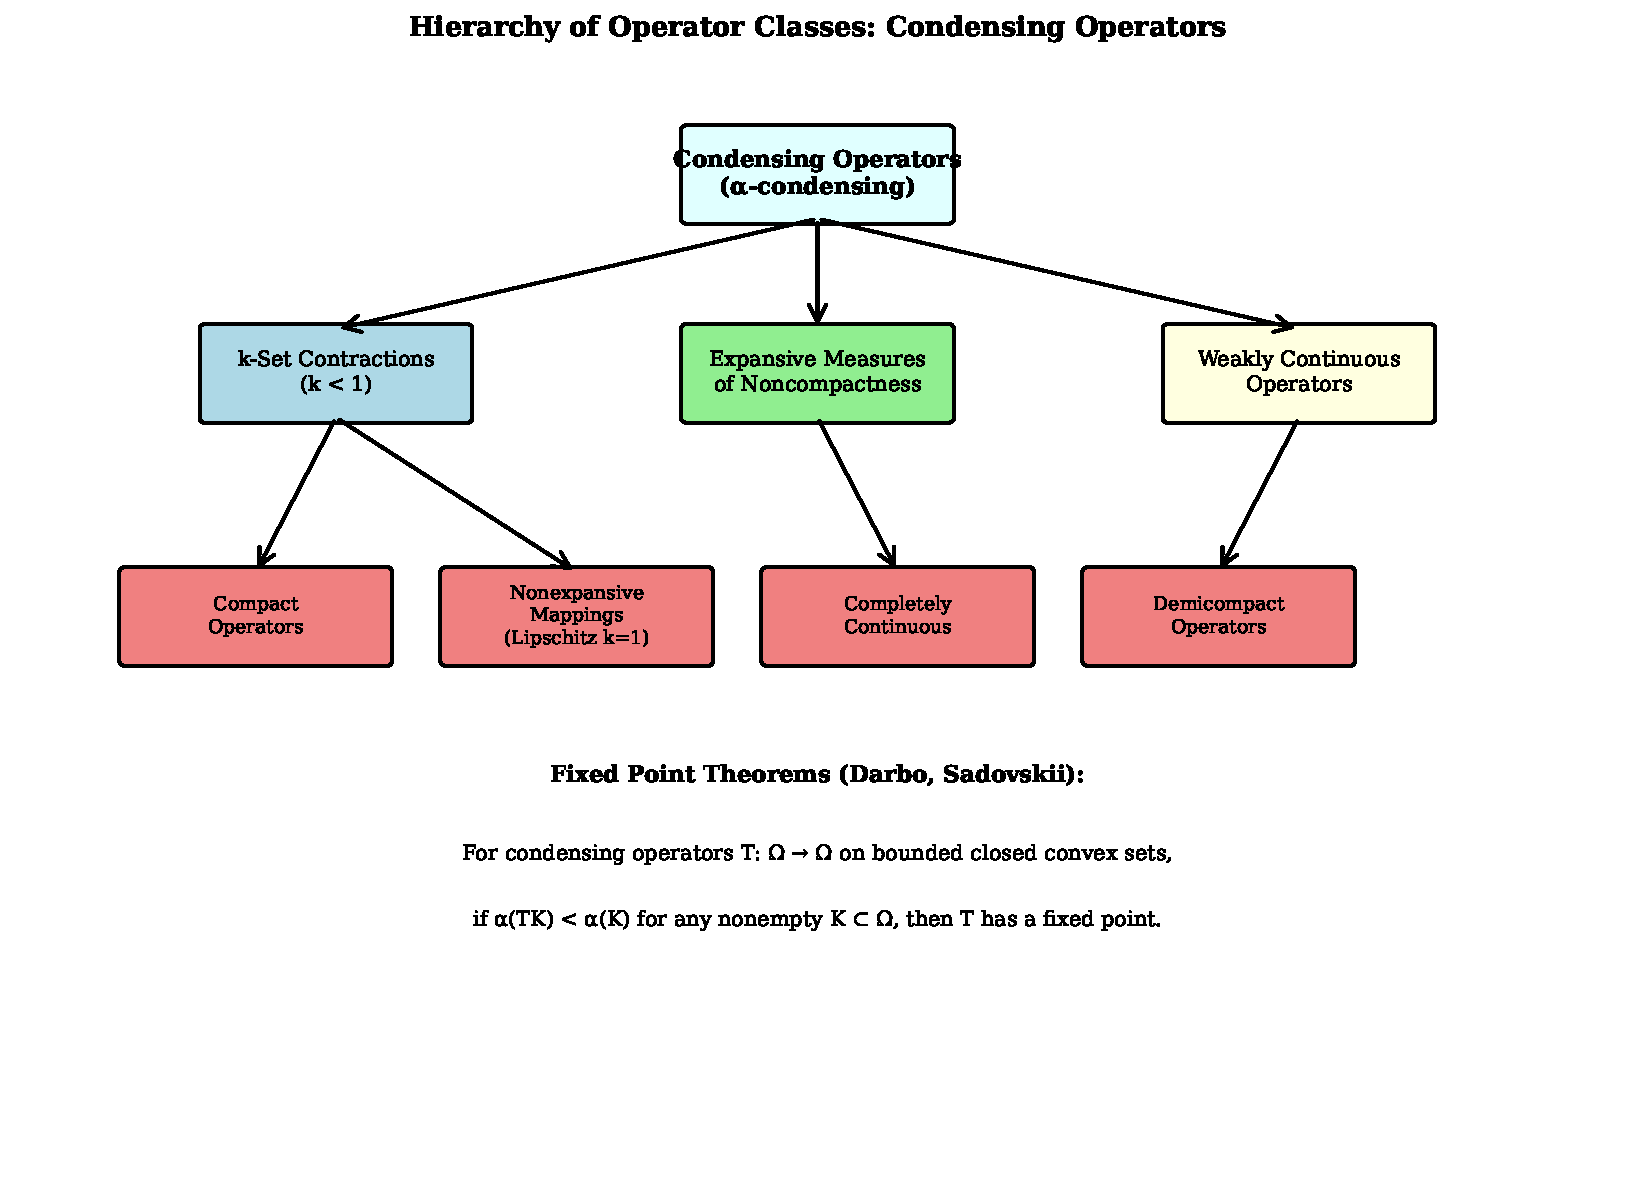
\includegraphics[width=0.85\textwidth]{fig_condensing_hierarchy}
\end{center}

\end{frame}

\begin{frame}{Sadovskii's Fixed Point Theorem}

\begin{theorem}[Sadovskii - Generalized Fixed Point Theorem]
Let $\Omega$ be a nonempty, bounded, closed and convex subset of a Banach space $X$, and let $T: \Omega \to \Omega$ be a continuous mapping. If $T$ is $\alpha$-condensing (where $\alpha$ is the measure of noncompactness), then $T$ has at least one fixed point in $\Omega$.
\end{theorem}

\vspace{0.3cm}

\textbf{Comparison with previous theorems:}
\begin{center}
\begin{tabular}{|l|c|c|c|}
\hline
\textbf{Theorem} & \textbf{Requirement} & \textbf{Operator Type} & \textbf{Conclusion} \\
\hline
Schauder & Compact $K$ & Continuous & FP exists \\
Banach & $\|Tx - Ty\| \leq k\|x-y\|$ & Contraction & Unique FP \\
Darbo & $\mu(T(X)) \leq k\mu(X)$ & k-set contract. & FP exists \\
Sadovskii & $\alpha(T(X)) < \alpha(X)$ & Condensing & FP exists \\
\hline
\end{tabular}
\end{center}

\end{frame}

\begin{frame}{Definition 6.18: Dhage's Concept}

\begin{definition}[D-Set-Lipschitz Mapping]
A mapping $T: X \to X$ is called \alert{D-set-Lipschitz} if there exists an upper semicontinuous nondecrasing function $\varphi: \mathbb{R}^+ \to \mathbb{R}^+$ with $\varphi(0) = 0$ such that:
\[
\mu(T(A)) \leq \varphi(\mu(A))
\]
for all $A \in \mathcal{B}(X)$ with $T(A) \subseteq B(X)$, where $\varphi(r) = kr$ defines a \textbf{k-set Lipschitz mapping} ($k > 0$).

If $k < 1$, then $T$ is a \textbf{k-set contraction}; if $\varphi(r) < r$ for $r > 0$, it is a \textbf{nonlinear D-set contraction}.
\end{definition}

\vspace{0.3cm}

\textbf{Remark 6.7 (Dhage):} Properties of D-functions:
\begin{itemize}
    \item If $\varphi, \psi$ are D-functions, then $i)\, \varphi + \psi$, $ii)\, \lambda\varphi$ ($\lambda > 0$), and $iii)\, \varphi \circ \psi$ are also D-functions
    \item Common D-functions: $\psi(r) = kr$, $\psi(r) = \frac{kr}{1+r}$, $\psi(r) = \log(1+r)$
\end{itemize}

\end{frame}

\begin{frame}{Theorem 6.28-6.29: Darbo-type Results}

\begin{theorem}[6.28 - Darbo's Generalization]
Let $\Omega$ be a nonempty, bounded, closed and convex subset of a Banach space $E$, and let $T: \Omega \to \Omega$ be a continuous mapping. If there exists a constant $k \in [0, 1)$ such that:
\[
\mu(T(X)) \leq k \mu(X)
\]
for any nonempty subset $X$ of $\Omega$ (where $\mu$ is the measure of noncompactness), then $T$ has a fixed point in $\Omega$.
\end{theorem}

\begin{theorem}[6.29 - Nonlinear D-Set Contraction (Dhage)]
Let $C$ be a closed, convex and bounded subset of a Banach space $X$, and let $T: C \to C$ be a continuous and nonlinear D-set contraction. Then $T$ has a fixed point.
\end{theorem}

\textbf{Proof idea:} Use the property that for a nonlinear D-function with $\varphi(r) < r$ for $r > 0$, the iterates $\varphi^n(t) \to 0$ as $n \to \infty$.

\end{frame}

\begin{frame}{Fixed Point Existence and Attractivity}

\textbf{Remark 6.8 - Attractivity of Fixed Points:}

If $\tilde{F}(T) = \{x \in C : Tx = x\}$ denotes the set of fixed points of $T: C \to C$, then:

\begin{enumerate}
    \item $\tilde{F}(T) \in \ker\mu$ (the set of fixed points has measure zero, i.e., is compact)
    \item If $\tilde{F}(T) \notin \ker\mu$, then $\mu(\tilde{F}(T)) > 0$ and we have $\mu(T(\tilde{F}(T))) = \mu(\tilde{F}(T))$
    \item From nonlinear set contractivity: $\mu(T(\tilde{F}(T))) \leq \varphi(\mu(\tilde{F}(T)))$
    \item Since $\varphi(r) < r$ for $r > 0$, this is a \textbf{contradiction}
    \item Therefore: $\tilde{F}(T) \in \ker\mu$ (i.e., $\tilde{F}(T)$ is compact)
\end{enumerate}

\vspace{0.3cm}

This particular property of measures has important applications to the \textbf{attractivity of solutions} in the study of nonlinear functional integral equations.

\end{frame}

% ============================================================================
\section{Applications and Examples}
% ============================================================================

\begin{frame}[fragile]{Example: Fixed Point via k-Set Contraction}

\textbf{Problem:} Find fixed points of $T: L^2[0, 1] \to L^2[0, 1]$ defined by:
\[
(Tx)(t) = \int_0^1 K(t, s) f(s, x(s)) \, ds
\]

where $K$ is a kernel and $f$ is a Carathéodory function.

\vspace{0.3cm}

\textbf{Approach using Darbo's theorem:}

\begin{lstlisting}
# Verify k-set contraction property
def verify_k_set_contraction(T, measured_sets, k=0.7):
    """
    Check if T is k-set contraction by estimating
    measure of noncompactness of image
    """
    results = []
    for A in measured_sets:
        TA = [T(x) for x in A]
        mu_A = measure_noncompactness(A)
        mu_TA = measure_noncompactness(TA)

        ratio = mu_TA / mu_A if mu_A > 0 else 0
        results.append({
            'set': A, 'mu_A': mu_A, 'mu_TA': mu_TA,
            'ratio': ratio, 'is_k_contract': ratio <= k
        })

    return all(r['is_k_contract'] for r in results), results

# If verified with k < 1, Darbo's theorem guarantees
# existence of fixed point in the domain
\end{lstlisting}

\end{frame}

\begin{frame}{Applications to Integral and Differential Equations}

\textbf{Application 1: Nonlinear Integral Equations}
\begin{itemize}
    \item Fredholm equations: $x(t) = f(t) + \int_a^b K(t,s) g(s, x(s)) \, ds$
    \item Using k-set contractions and condensing operators to establish existence
\end{itemize}

\vspace{0.3cm}

\textbf{Application 2: Evolution Equations in Banach Spaces}
\begin{itemize}
    \item Partial differential equations with nonlinear lower-order terms
    \item Skrypnik degree theory for pseudomonotone operators $A: H^1 \to H^{-1}$
\end{itemize}

\vspace{0.3cm}

\textbf{Application 3: Fixed Point Sequences}
\begin{itemize}
    \item When fixed points are not unique, study the structure of $\tilde{F}(T) = \{x : Tx = x\}$
    \item Attractivity properties: if $\tilde{F}(T)$ is nonempty, it must be compact
\end{itemize}

\vspace{0.3cm}

\textbf{Application 4: Variational Inequalities}
\begin{itemize}
    \item Find $x \in K$ such that $\langle Ax, v - x \rangle \geq 0$ for all $v \in K$
    \item Use Skrypnik degree or condensing operator theory
\end{itemize}

\end{frame}

\begin{frame}{Summary and Key Takeaways}

\textbf{Chapter 6 Main Results:}

\begin{enumerate}
    \item \textbf{Invariance Principles (6.2):} Degree theory is independent of Banach space choice under suitable conditions

    \item \textbf{Skrypnik Degree (6.3):} Extends finite-dimensional degree to pseudomonotone operators on reflexive spaces
    \begin{itemize}
        \item Handles operators mapping $X \to X^*$
        \item Based on finite-dimensional approximations
    \end{itemize}

    \item \textbf{k-Set Contractions (6.4):} Use measure of noncompactness $\mu$ instead of pointwise distances
    \begin{itemize}
        \item Darbo's Theorem: $\mu(T(X)) \leq k\mu(X)$ with $k < 1 \Rightarrow$ fixed point exists
        \item Generalizes Banach Contraction Principle
    \end{itemize}

    \item \textbf{Condensing Operators (6.5):} Even broader class than k-set contractions
    \begin{itemize}
        \item Sadovskii's theorem: condensing operators have fixed points
        \item Applications to differential and integral equations
    \end{itemize}
\end{enumerate}

\end{frame}

\begin{frame}{Connection to Previous Chapters}

\textbf{Fixed Point Theorems Hierarchy:}

\begin{enumerate}
    \item \textbf{Chapter 2:} Banach Contraction Mapping (complete metric spaces, unique FP)
    \item \textbf{Chapter 3:} Nonexpansive and quasi-nonexpansive mappings
    \item \textbf{Chapter 4:} Iterative methods (Mann, Ishikawa, Noor iterations)
    \item \textbf{Chapter 5:} Schauder, Brouwer fixed point theorems (topological methods)
    \item \textbf{Chapter 6:} Degree theory, condensing operators, measure-theoretic approaches
\end{enumerate}

\vspace{0.5cm}

\textbf{Progression:} Pointwise distance $\to$ Topological degree $\to$ Measure of noncompactness $\to$ Condensing operators

\vspace{0.5cm}

\textbf{Future chapters:} These tools apply to variational inequalities, differential equations, and integral equations (Chapters 8--9).

\end{frame}

\begin{frame}[fragile]{References and Further Reading}

\textbf{Key papers cited in Chapter 6:}
\begin{itemize}
    \item \textbf{[564]} Skrypnik, I.V., 1973. Nonlinear elliptic equations of higher order
    \item \textbf{[155]} Darbo, G., 1955. Punti uniti in trasformazioni a codominio non compatto
    \item \textbf{[175]} Dhage, B.C., Various works on D-set-Lipschitz mappings and fixed points
    \item \textbf{[176]} Dhage, B.C., Properties of D-functions in condensing operators
\end{itemize}

\vspace{0.4cm}

\textbf{Recommended further study:}
\begin{enumerate}
    \item Degree theory in infinite dimensions: See Chapter 6.2--6.3
    \item k-Set contractions: Darbo (1955), generalized by many
    \item Measure of noncompactness: Kuratowski, Hausdorff measures
    \item Applications: See Chapters 8 (differential equations), 9 (integral equations)
\end{enumerate}

\end{frame}

\end{document}
